\let\negmedspace\undefined
\let\negthickspace\undefined

\documentclass[journal,12pt,onecolumn]{IEEEtran}
%\documentclass[journal,12pt,twocolumn]{IEEEtran}
%
\usepackage{setspace}
\usepackage{gensymb}
%\doublespacing
\singlespacing

%\usepackage{graphicx}
%\usepackage{amssymb}
%\usepackage{relsize}
\usepackage[cmex10]{amsmath}
%\usepackage{amsthm}
%\interdisplaylinepenalty=2500
%\savesymbol{iint}
%\usepackage{txfonts}
%\restoresymbol{TXF}{iint}
%\usepackage{wasysym}
\usepackage{amsthm}
\usepackage{mathrsfs}
\usepackage{txfonts}
\usepackage{stfloats}
\usepackage{cite}
\usepackage{cases}
\usepackage{subfig}
%\usepackage{xtab}
\usepackage{longtable}
\usepackage{multirow}
%\usepackage{algorithm}
%\usepackage{algpseudocode}
\usepackage{enumitem}
\usepackage{mathtools}
\usepackage{tikz}
\usepackage{circuitikz}
\usepackage{verbatim}
\usepackage{hyperref}
%\usepackage{stmaryrd}
\usepackage{tkz-euclide} % loads  TikZ and tkz-base
%\usetkzobj{all}
\usepackage{listings}
\usepackage{color}                                            %%
\usepackage{array}                                            %%
\usepackage{longtable}                                        %%
\usepackage{calc}                                             %%
\usepackage{multirow}                                         %%
\usepackage{hhline}                                           %%
\usepackage{ifthen}                                           %%
%optionally (for landscape tables embedded in another document): %%
\usepackage{lscape}     
\usepackage{multicol}
\usepackage{chngcntr}
\usepackage{iftex}
%\usepackage[latin9]{inputenc}
\usepackage{geometry}
\usepackage{bm}
%\geometry{verbose,tmargin=2cm,bmargin=3cm,lmargin=1.8cm,rmargin=1.5cm,headheight=2cm,headsep=2cm,footskip=3cm}
\usepackage{array}
\newcolumntype{L}[1]{>{\raggedright\let\newline\\\arraybackslash\hspace{0pt}}m{#1}}
\newcolumntype{C}[1]{>{\centering\let\newline\\\arraybackslash\hspace{0pt}}m{#1}}
\newcolumntype{R}[1]{>{\raggedleft\let\newline\\\arraybackslash\hspace{0pt}}m{#1}}

%\usepackage{graphicx}
%\usepackage{setspace}
%\usepackage{parskip}

\def \hsp {\hspace{3mm}}

\makeatletter

\providecommand{\tabularnewline}{\\}



\makeatother
\ifxetex
\usepackage[T1]{fontenc}
\usepackage{fontspec}
%\setmainfont[ Path = fonts/]{Sanskrit_2003.ttf}
\newfontfamily\nakulafont[Script=Devanagari,AutoFakeBold=2,Path = fonts/]{Nakula}
%\newfontfamily\liberationfont{Liberation Sans Narrow}
%\newfontfamily\liberationsansfont{Liberation Sans}
\fi
\usepackage{tikz}
\usepackage{xcolor}
%\usepackage{enumerate}

%\usepackage{wasysym}
%\newcounter{MYtempeqncnt}
\DeclareMathOperator*{\Res}{Res}
%\renewcommand{\baselinestretch}{2}
\renewcommand\thesection{\arabic{section}}
\renewcommand\thesubsection{\thesection.\arabic{subsection}}
\renewcommand\thesubsubsection{\thesubsection.\arabic{subsubsection}}

\renewcommand\thesectiondis{\arabic{section}}
\renewcommand\thesubsectiondis{\thesectiondis.\arabic{subsection}}
\renewcommand\thesubsubsectiondis{\thesubsectiondis.\arabic{subsubsection}}

% correct bad hyphenation here
\hyphenation{op-tical net-works semi-conduc-tor}
\def\inputGnumericTable{}                                 %%

\lstset{
	language=tex,
	frame=single, 
	breaklines=true
}

%\begin{document}
%


\newtheorem{theorem}{Theorem}[section]
\newtheorem{problem}{Problem}
\newtheorem{proposition}{Proposition}[section]
\newtheorem{lemma}{Lemma}[section]
\newtheorem{corollary}[theorem]{Corollary}
\newtheorem{example}{Example}[section]
\newtheorem{definition}[problem]{Definition}
%\newtheorem{thm}{Theorem}[section] 
%\newtheorem{defn}[thm]{Definition}
%\newtheorem{algorithm}{Algorithm}[section]
%\newtheorem{cor}{Corollary}
\newcommand{\BEQA}{\begin{eqnarray}}
	\newcommand{\EEQA}{\end{eqnarray}}
\newcommand{\define}{\stackrel{\triangle}{=}}
\bibliographystyle{IEEEtran}
%\bibliographystyle{ieeetr}
\providecommand{\mbf}{\mathbf}
\providecommand{\pr}[1]{\ensuremath{\Pr\left(#1\right)}}
\providecommand{\qfunc}[1]{\ensuremath{Q\left(#1\right)}}
\providecommand{\sbrak}[1]{\ensuremath{{}\left[#1\right]}}
\providecommand{\lsbrak}[1]{\ensuremath{{}\left[#1\right.}}
\providecommand{\rsbrak}[1]{\ensuremath{{}\left.#1\right]}}
\providecommand{\brak}[1]{\ensuremath{\left(#1\right)}}
\providecommand{\lbrak}[1]{\ensuremath{\left(#1\right.}}
\providecommand{\rbrak}[1]{\ensuremath{\left.#1\right)}}
\providecommand{\cbrak}[1]{\ensuremath{\left\{#1\right\}}}
\providecommand{\lcbrak}[1]{\ensuremath{\left\{#1\right.}}
\providecommand{\rcbrak}[1]{\ensuremath{\left.#1\right\}}}
\theoremstyle{remark}
\newtheorem{rem}{Remark}
\newcommand{\sgn}{\mathop{\mathrm{sgn}}}
\providecommand{\abs}[1]{\left\vert#1\right\vert}
\providecommand{\res}[1]{\Res\displaylimits_{#1}} 
\providecommand{\norm}[1]{\left\lVert#1\right\rVert}
%\providecommand{\norm}[1]{\lVert#1\rVert}
\providecommand{\mtx}[1]{\mathbf{#1}}
\providecommand{\mean}[1]{E\left[ #1 \right]}
\providecommand{\fourier}{\overset{\mathcal{F}}{ \rightleftharpoons}}
%\providecommand{\hilbert}{\overset{\mathcal{H}}{ \rightleftharpoons}}
%\providecommand{\system}{\overset{\mathcal{H}}{ \longleftrightarrow}}
\providecommand{\system}[1]{\overset{\mathcal{#1}}{ \longleftrightarrow}}
\providecommand{\gauss}[2]{\mathcal{N}\ensuremath{\left(#1,#2\right)}}
%
%\newcommand{\solution}[2]{\textbf{Solution:}{#1}}
\newcommand{\solution}{\noindent \textbf{Solution: }}
\newcommand{\cosec}{\,\text{cosec}\,}
\newcommand{\sinc}{\,\text{sinc}\,}
\newcommand{\rect}{\,\text{rect}\,}
\providecommand{\dec}[2]{\ensuremath{\overset{#1}{\underset{#2}{\gtrless}}}}
\newcommand{\myvec}[1]{\ensuremath{\begin{pmatrix}#1\end{pmatrix}}}
\newcommand{\mydet}[1]{\ensuremath{\begin{vmatrix}#1\end{vmatrix}}}
\newcommand*{\permcomb}[4][0mu]{{{}^{#3}\mkern#1#2_{#4}}}
\newcommand*{\perm}[1][-3mu]{\permcomb[#1]{P}}
\newcommand*{\comb}[1][-1mu]{\permcomb[#1]{C}}
%\numberwithin{equation}{section}
\numberwithin{equation}{section}
%\numberwithin{problem}{section}
%\numberwithin{definition}{section}
\makeatletter
\@addtoreset{figure}{problem}
\makeatother
%\let\StandardTheFigure\thefigure
\let\vec\mathbf
%\renewcommand{\thefigure}{\theproblem.\arabic{figure}}
\renewcommand{\thefigure}{\arabic{section}.\arabic{figure}}
%\setlist[enumerate,1]{before=\renewcommand\theequation{\theenumi.\arabic{equation}}
	%\counterwithin{equation}{enumi}
	%\renewcommand{\theequation}{\arabic{subsection}.\arabic{equation}}
\let\StandardTheFigure\thefigure
	\vspace{3cm}
	%\usepackage{babel}
	\begin{document}
		\title{ K-NN Machine Learning Alogorithm}
		\author{ Mannem Charan AI21BTECH11019}
                \maketitle
		\begin{abstract}
			This report consists of my basic understanding of one of the popular Ml methods "K-NN".
		\end{abstract}
               \section{K-NN}
                 K-NN,K-Nearest Neighbour algorithm is one of the simplest machine learning technique and it comes under supervised learning.It will not assume any relationship between dependent and independent variables so it is a non-parametric machine learning algorithm.It is also known as "Lazy-learning" algorithm beause it doesn't have any training phase, it will just store the training data and uses it at the time of classification.
	       \section{Understanding K-NN}
	       The K-NN algorithm \textbf{assumes} similarity between the new data and the available data and then it will put the new data by comparing similarity between the available categories.The name K-Nearest Neighbours signifies that we try to compare the new data point with "k" nearest neighbours. And we will define neighbour by measuring the euclidian distance between the data points.So K-NN uses every input instances of the data to classify the new data. In case of Regression we try to take mean or median of labels of the "k" nearest neighbours.So our job is to store the complete training data and take a new data point find the "k" nearest neighbours(by\, euclidian\, distance\, method) and if it is classifcation take the category/label of majority neighbours or else take the mean/median of continuos values of "k" nearest neighbours.So the important thing here is, choosing the value of "k".
	       \section{Choosing the k}
	       As you know that, "k" here represent the number closest data points we are taking for comparing the similarities with the new data point.So choosing "k" affects the performance of the model, we can study the changes in model with "k" using error curves shown in Fig $\ref{Fig 1}$.
	       \begin{figure}
		 \centering
		 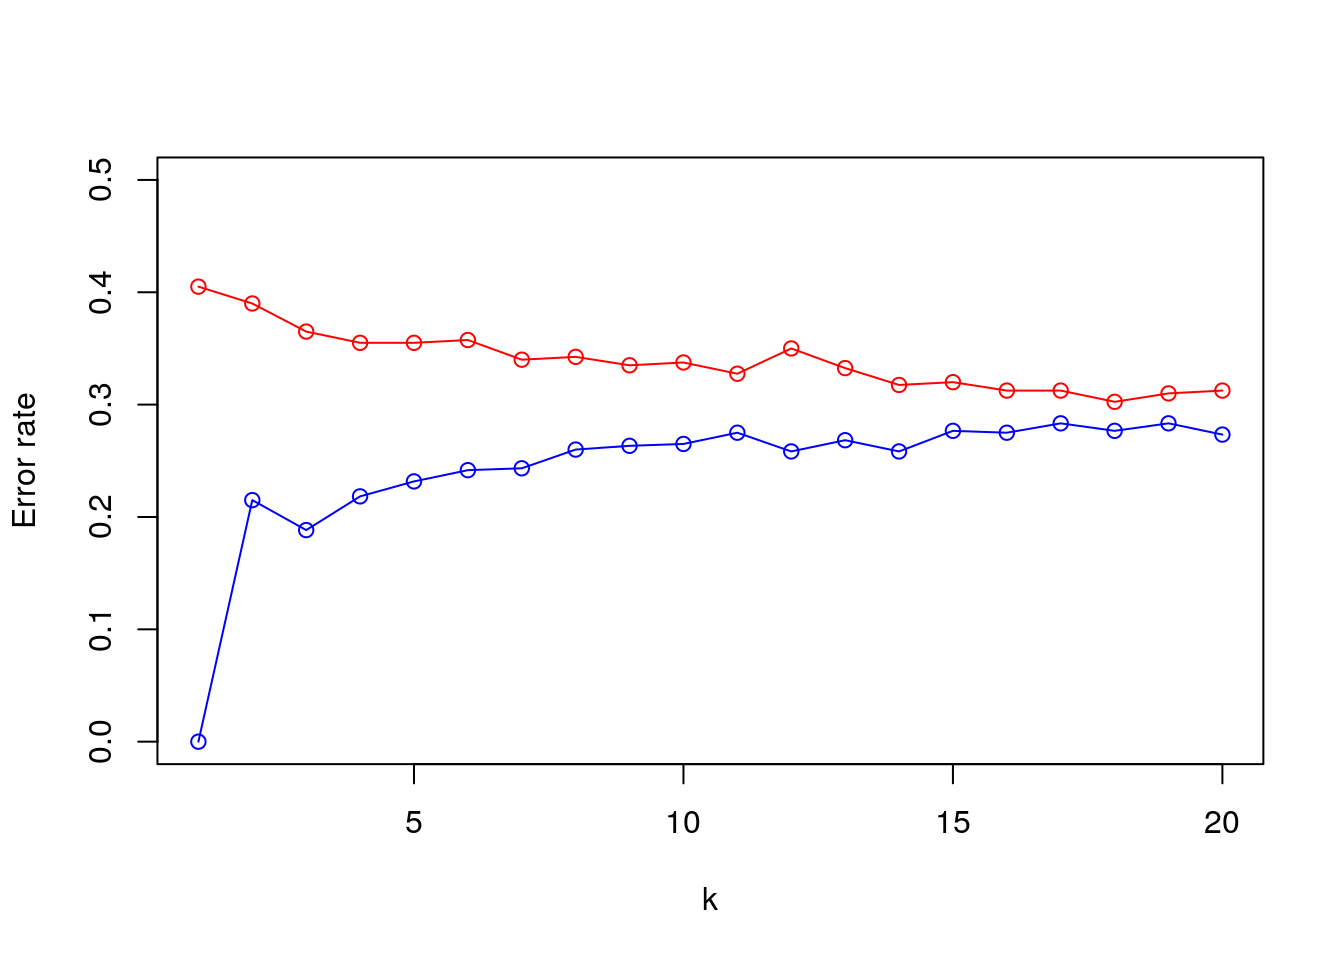
\includegraphics[width = 10cm]{errorcurve.png}
		 \caption{error rates w.r.t $k$}
		 \label{Fig 1}
	       \end{figure}
       The red line reperesnts the test error and blue line represents the train error.So for $K=1$,the training error is $0$ this can be understood since for every data point the nearest point is the point itself.But the test error is high for $k=1$ due to the noise in the data which leads to overfitting.In general, as k increases the 
	the test error will decrease with increase in train error.So there is no exact approach to choose $k$ some data scientists prefer to choose a odd number if there are two classes and another simple way is take $k =\sqrt{N}$ where $N$ are the total data samples in training dataset.
	       \section{Advantages of K-NN}
	        \begin{enumerate}
		 \item It is easy to understand and implement
	         \item It is not sensitive to the outliers(by\, choosing\, correct\, value\, of\, $k$)
	         \item It is more efficient for large datasets.
	         \item It takes no time to train for obvious reasons.
	        \end{enumerate}
	       \section{Disadvantages of K-NN}
	        \begin{enumerate}
		 \item K-NN gives equal importance to all features, as it is only takes distance between two data points.
	         \item Uses lot of computational power.
	        \end{enumerate}
	       \section{Data Preparation for K-NN}
	        \begin{enumerate}
		 \item \textbf{Feature Scaling:}Proper feature scaling is required, since we are taking distance between the points as the measure to say closeness,it would be better if all the features are in the same scale.
		 \item \textbf{Dimensionality Reduction :} If there are more classes to classify, then it is not a good judgement to take class of majority neighbours.So using dimensionality reducion techniques like feature selection helps k-NN to work more accurately.
	         \item \textbf{Missing Features :} We can't use k-NN if we don't have the data of all features for all data samples(as\, we\, can't\, find\, the\, norm),so either we have to delete the samples not having all features,or we have to predict the missing features(imputation).
		\end{enumerate}
	       \section{Questions}
	        \begin{enumerate}
		 \item Why k-NN is known as lazy-learning algorithm?
		 \item What is "k" in k-NN algorithm?
		 \item How the model changes with the "k" value?
		 \item What is the measure we are using in k-NN to find the closeness between the data points?
		 \item Mention the data preprocessing steps used in k-NN?
	        \end{enumerate}
	       \section{Solutions}
	        \begin{enumerate}
		 \item Because in k-NN we only storing the training data there is no training phase.
		 \item The "k" represents the the number of closest neighbours we are taking in the algorithm.
		 \item For the lower values of "k", there is a high chance of overfitting and as we increase k the generalization error decreases.
		 \item In general we use euclidean distance as measure to find the closeness between the data points.
		 \item The important data pre-processing steps that must be done in k-NN are,
			  \begin{itemize}
			    \item Feature Selection
			    \item Feature Scaling
			    \item Imputation/deleting the missing features.
			  \end{itemize}
		\end{enumerate}
         \end{document}
